\chapter{Pronunciation and overall quality similarity measures}\label{chap:similarity_pronunciation}

Pronunciation and overall quality similarities measurement is a subtask in singing voice assessment. which is useful in the online singing training scenario to assess the pronunciation quality and the overall quality of the student's singing. In the last chapter, we have discussed the possibility of using computational models to detect the mispronunciation syllables in jingju singing. However, as we have mentioned in \secref{sec:ch3:char_singing}, in some cases, although the student does not commit any mispronunciation, there still exists a clear gap on pronunciation and overall quality between the singing of teacher and student. The rigour of the jingju singing training and the learning by imitation training method require the student, especially the professional one, to imitate the timbre quality of the jingju master. Thus, a system which can measure the pronunciation and overall quality similarities between the singing of teacher and student is a useful component of the automatic system for jingju singing assessment.

In the context of this dissertation, pronunciation and overall quality similarities measurement aims to measure the pronunciation and overall quality similarities between the teacher and student's corresponding phoneme segments. This chapter aims to address the pronunciation and overall quality similarities measurement task in the context of jingju singing training, presenting several methods and an evaluation of these methods. The main goal of this chapter are:

\begin{enumerate}[leftmargin=*]
\item To address the similarity measure problem for jingju singing. The problem is formulated as building machine learning models to perform phoneme embedding regarding pronunciation and overall quality aspects. Several neural network architectures are experimented to address this problem.

\item To present a description of the classification model for phoneme embedding, and to explore the siamese network model for the same purpose.

\item To present an evaluation of the classification model and the siamese model.
\end{enumerate}

\section{Task description}

Task description of the pronunciation and overall quality similarities measurement in this section is continued building on the problem formulation presented in \secref{sec:ch3:similarity_formulation}.

Given the singing audio recording pre-segmented into phoneme-level, the most relevant task is to develop the computational models which can measure the pronunciation and overall quality similarities between phoneme segments. We constrain the granularity at phoneme-level because it is the smallest pronunciation unit in jingju singing teacher, and it is also the basic component to constitute the high-level singing unit, such as syllable and phrase. In the context of this thesis, we mainly consider using phoneme embedding to distill the pronunciation and overall quality information of the phoneme segment, then apply distance measures to define the similarity between two segments. The advantages of using phoneme embedding rather than the traditional sequential alignment method for the similarity measures have been discussed in \secref{sec:ch3:similarity_formulation}. We adopt deep learning-based methods for generating phoneme embeddings from variable-length phoneme segments. The deep learning-based classification model aims to classify the phoneme segment into phoneme and overall quality categories. The output of the second last layer of the classification model will be used as the embedding. As an exploration, we also experiment the siamese network architecture for phoneme embedding learning task since this architecture was designed for measuring similarity between multiple inputs. Then, the similarity between two phoneme segments can be obtained by calculating the distance measure of their phoneme embeddings. Differ from the last chapter, we will evaluate the model performance directly on the manually pre-segmented phoneme segments rather than involving any automatic phoneme segmentation step into the pipeline. Thus, we leave the joint evaluation of phoneme segmentation and similarity measure for future work.

The two main tasks in this chapter are setting up the classification phoneme embedding model, proposing several improvements, and explore the siamese phoneme embedding model. The performance of these two tasks will be evaluated on \gls{POQSM} test dataset. The results of the two models will be discussed in detail.

\section{Baseline phoneme embedding networks}

We introduce a phoneme embedding neural network as the baseline model, which is able to convert variable-length phoneme segments into fixed-length vectors. We use the logarithmic Mel (log-mel) spectrogram of the phoneme segment as the input. The frame size and hop size of the spectrogram are respectively 46.4ms (2048 samples) and 10ms (441 samples). The low and high-frequency bounds of the Mel bank filters are 27.5Hz and 16kHz. This input representation is similar as we have been mentioned in \secref{sec:ch6:discriminative_model_method}.

\subsection{Fully-supervised classification network}

We call this network the fully-supervised classification network, because we use fully-supervised training method and provide to the network the phoneme class label for the pronunciation classification, or the professional/amateur binary label for the overall quality classification. Figure \ref{fig:ch7:classification_net} shows a diagram of this network. The main part of the network is a single or multi recurrent layers. The optimal layer number will be decided in the \secref{sec:ch7:baseline_results_classification}. The last layer of the network use softmax units for the categorical classification. We take the output vector from the last layer as the embedding - either a 27 dimensional vector for the pronunciation embedding (figure \ref{fig:ch7:classification_net} left part) or a 2 dimensional vector for the overall quality embedding (figure \ref{fig:ch7:classification_net} right part). We use categorical cross-entropy loss during the network training. The embeddings learned by this network are expected to capture either the pronunciation or overall quality characteristics of the phoneme segment. We also experimented sharing the weights between the left and right branches of the architecture, so that we could use one network to learn both pronunciation and overall quality embeddings, which is the idea of multi-task learning \cite{ruder2017overview}. However, our experiment shows that it doesn't work better than individual task learning.

\begin{figure}[ht!]
    \centering
    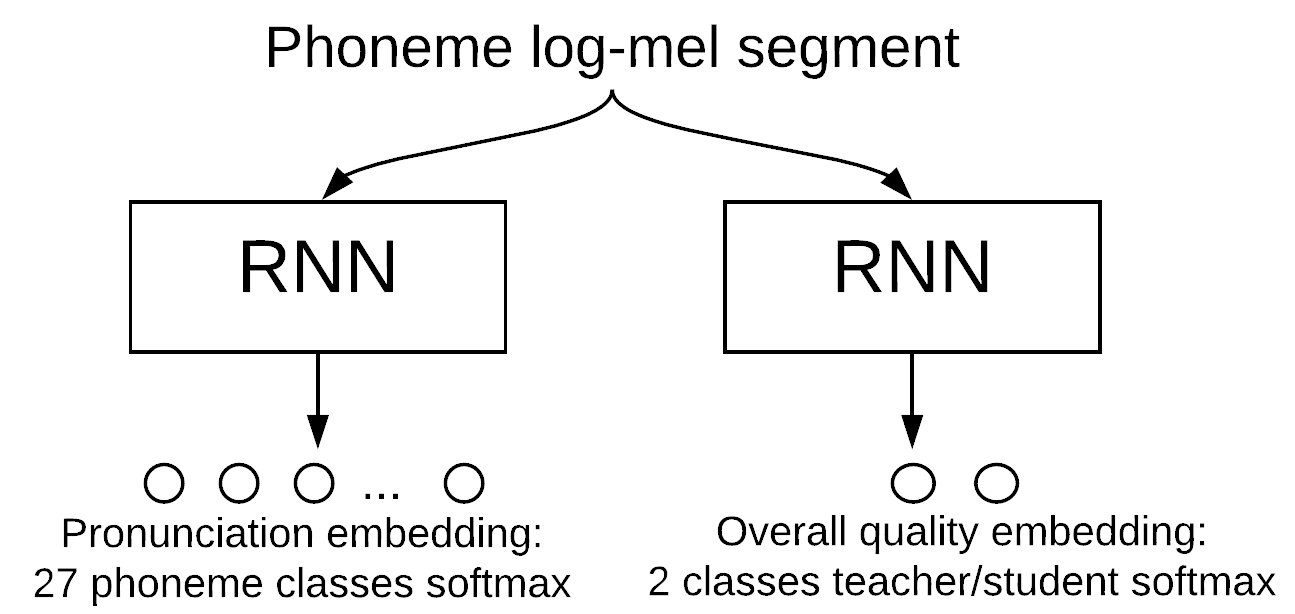
\includegraphics[width=0.7\textwidth]{figs/ch7/classification_net.png}
    \caption{Fully-supervised classification phoneme embedding network for learning pronunciation (left part) or overall quality (right part) embeddings. \gls{RNN}: recurrent network network.}
    \label{fig:ch7:classification_net}
\end{figure}

\subsection{Model training}

The weights of the network are learned with mini-batch training (batch size 64), adam \cite{kingma2014adam} update rule and early stopping of 15 epochs. To accelerate the network training, we bucket the training phoneme segments which have a similar frame length into the same mini-batch. The segments are then zero-padded so that they have the same length as the longest segment of the mini-batch. 

\subsection{Experimental setup}\label{sec:ch7:experimental_setup_classification}

We use \gls{POQSM} test dataset presented in \secref{sec:ch4:poqsm_dataset} for the evaluation purpose. The train, validation and test split of this dataset can be consulted in \tabref{tab:ch4:exp_dataset_poqsm}.

For the pronunciation aspect, we measure the cosine similarity for every phoneme embedding pair in the test set. The ground truth label of an embedding pair is 1 if they belong to the same phoneme class, or 0 vice versa. For overall quality aspect, we only measure the cosine similarity of the phoneme embedding pairs of the same phoneme class. The ground truth label is 1 if two embeddings belong to the same overall quality class -- professional or amateur, 0 vice versa. We report the \gls{AP} between the cosine similarities and the ground truth as the evaluation metric. The \gls{AP} is used previously to evaluate speech word acoustic embedding \cite{Kampera,Settle2016a}. It is also suggested as the metric for imbalanced test set \cite{Davis2006}, which is the case of the pronunciation aspect evaluation.

We experiment 9 \gls{RNN} architectures of \gls{BiLSTM} recurrent layer and fully-connected layer combinations and report their \gls{AP} on the validation set. Each recurrent layer is bidirectional with 32 \gls{DNN} units in each direction (\gls{BiLSTM}). Each fully-connected layer has 64 \gls{ReLU} activation units and followed by a dropout layer with 0.5 dropout rate. We train each model 5 times with different random seeds, and take the mean value of the average precisions. Two optimal architectures are decided separately for pronunciation embedding and overall quality embedding. Finally, we evaluate the performance of the optimal architectures on the test set.

\subsection{Results and discussion of the baseline}\label{sec:ch7:baseline_results_classification}

Table \ref{tab:ch7:validation_classification} shows the \gls{AP} results on the validation set for 9 different architectures. We observe that fully-connected layer doesn't help increase the \gls{AP}. The pronunciation and overall quality aspects reach their highest \gls{AP} respectively by using 2 \gls{BiLSTM} layers and 1 \gls{BiLSTM} layer. 

\begin{table}[ht!]
\centering
\caption{Mean value of average precision on the validation set over 5 runs, using classification network embedding. R: \# recurrent layers, F: \# fully-connected layers.}
\label{tab:ch7:validation_classification}
\begin{tabular}{llcc}
\toprule
R & F & Pronunciation AP & Overall quality AP \\
\midrule
1 & 0 & 0.690            & \textbf{0.934}     \\
1 & 1 & 0.694            & 0.926              \\
2 & 0 & \textbf{0.695}   & 0.915              \\
2 & 1 & 0.694            & 0.928              \\
2 & 2 & 0.689            & 0.927              \\
3 & 0 & 0.691            & 0.924              \\
3 & 1 & 0.695            & 0.920              \\
3 & 2 & 0.684            & 0.924              \\
3 & 3 & 0.673            & 0.920             \\
\bottomrule
\end{tabular}
\end{table}

\begin{table}[ht!]
\centering
\caption{Average precision on the test set over 5 runs, using optimal network architectures.}
\label{tab:ch7:baseline_test}
\begin{tabular}{cc}
\toprule
Pronunciation AP & Overall quality AP \\
\midrule
0.645            & 0.632     \\
\bottomrule
\end{tabular}
\end{table}

Table \ref{tab:ch7:baseline_test} shows the evaluation results for the baseline classification network with the optimal architectures on the test set. We observe that the classification network test \gls{AP} is much worse than the validation \gls{AP} -- a 0.302 difference. We have two assumptions to explain this observation:

\textbf{Assumption i}: the test set amateur phoneme segments are very different from those of amateur train and validation sets, and similar to the professional segments. 

\textbf{Assumption ii}: the model is heavily overfitted on the train and validation sets.

We have the assumption i because the amateur part of the test set is special, which is recorded by the adult singers. However, the amateur segments in the train and validation sets are recorded mostly by primary school students. To show that the learned overall quality embeddings are not able to discriminate between professional and test set amateur phoneme segments for some phoneme classes, we use \gls{t-SNE} technique \cite{VanDerMaaten2008} to project the embeddings of three different groups -- professional embeddings, amateur train and validation embeddings and amateur test embeddings into a 2-dimensional space.

\begin{figure}
    \centering
    \subfloat[Non-voiced consonant phoneme class]{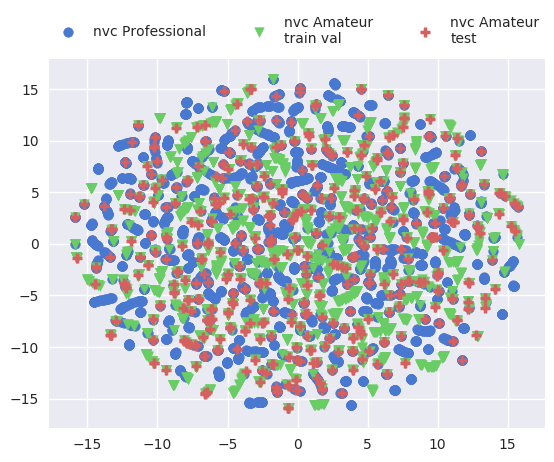
\includegraphics[width=0.475\textwidth]{figs/ch7/nvc_nodense.png}\label{fig:ch7:tsne_nodense_nvc}}
    \subfloat[Phoneme O class]{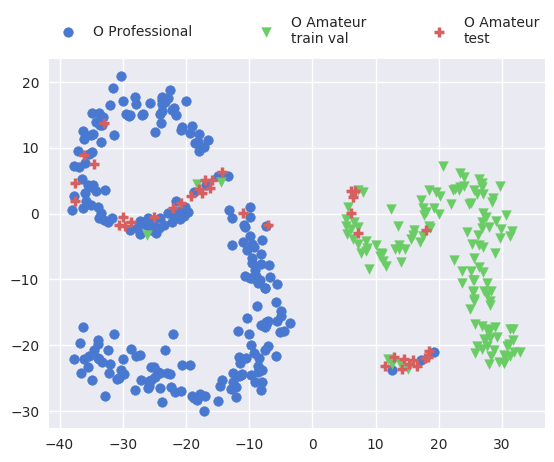
\includegraphics[width=0.475\textwidth]{figs/ch7/O_nodense.png}\label{fig:ch7:tsne_nodense_o}}
    \caption[]{t-SNE projection of classification network phoneme embeddings for overall quality aspect. nvc: non-voiced consonant; Blue dots: phoneme embeddings of the professional singers; Green triangles: training and validation sets phoneme embeddings of the amateur singers; Red plus: test set phoneme embeddings of the amateur singers.}
    \label{fig:ch7:tsne_nodense}
\end{figure}
    
Figure \ref{fig:ch7:tsne_nodense} shows two examples of \gls{t-SNE} projection for two phoneme classes -- non-voiced consonant and phoneme O, of which the test set \gls{AP}s are 0.626 and 0.677. For the non-voiced consonant class, we can't observe three separated groups of phoneme embeddings on figure \ref{fig:ch7:tsne_nodense_nvc}. For the phoneme O class of figure \ref{fig:ch7:tsne_nodense_o}, we can observe a clear separation between the professional phoneme segments (blue dots) and the amateur train and validation sets segments (green triangles). However, many amateur test set segments (red plus) are mixed up within the professional cluster. 

The mixing up of the test set amateur segments with the professional ones doesn't necessarily mean that these amateur test set phoneme segments have reached the professional singing quality, but perhaps we haven't learned a suitable phoneme embedding to distinguish them. To check if the amateur test segments can be discriminated from the professional segments by using acoustic features, we conduct a feature analysis. We first extract 151 features for the segments of the three groups using Essentia FreesoundExtractor\footnote{\url{http://essentia.upf.edu/documentation/freesound\_extractor.html}\label{foot:freesound}}. The feature name list can be checked online\footref{foot:zenodo_dlfm2018}.
Then we compute \gls{ANOVA} F-value for each feature, and sort the F-values to select the best individual features which are capable to separate between the three groups \cite{Stollera}. We use \texttt{f\_classif} function in scikit-learn python package to compute the \gls{ANOVA} F-value. Figure \ref{fig:ch7:feature_nvc} and figure \ref{fig:ch7:feature_o} shows the value distributions of individual feature for phoneme classes -- non-voiced consonant and O. 

\begin{figure}
    \centering
    \subfloat[Max der before max]{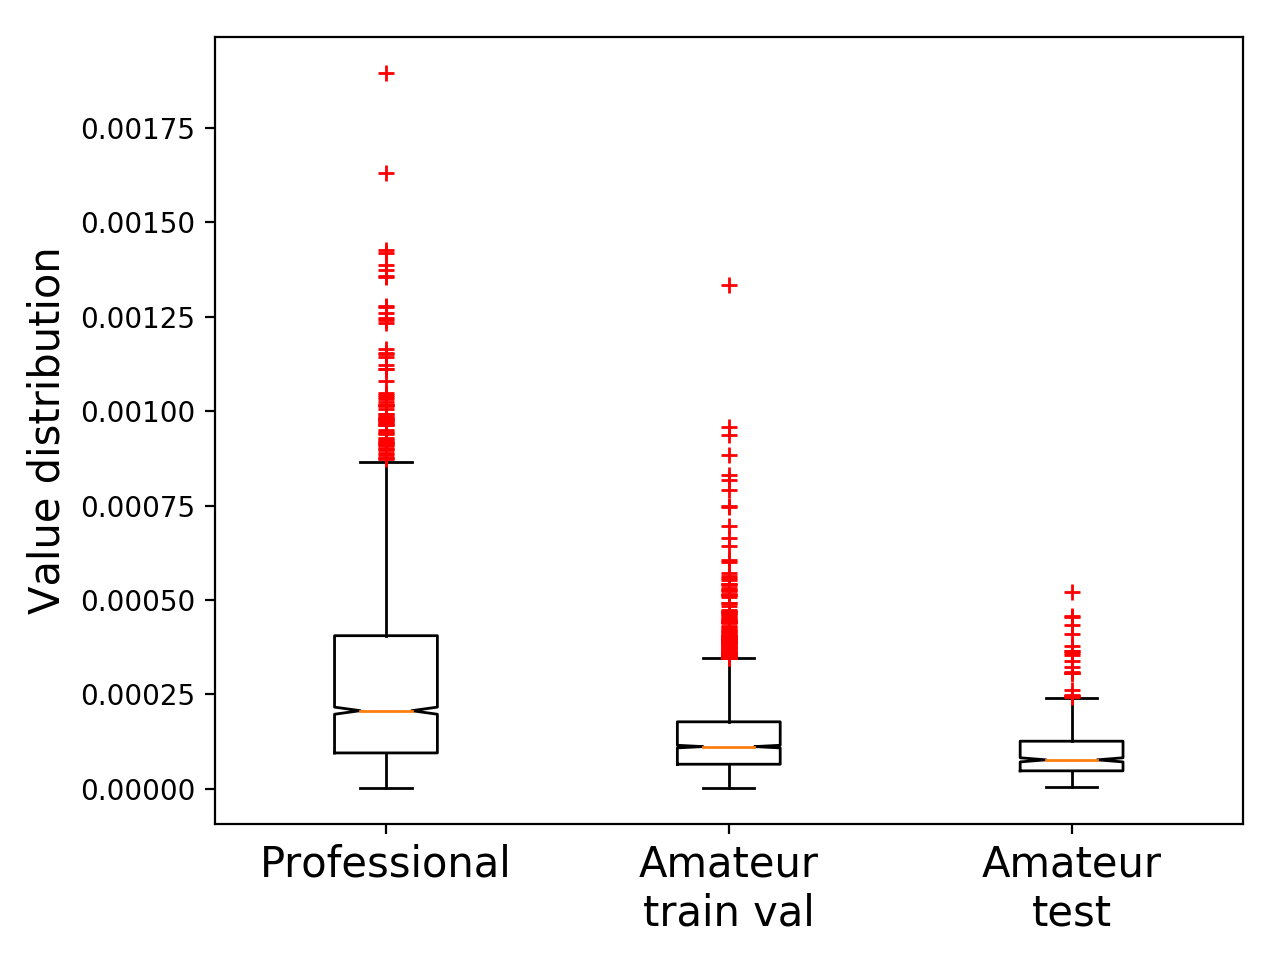
\includegraphics[width=0.475\textwidth]{figs/ch7/nvc_4_sfx_max_der_before_max.png}}
    \subfloat[ERB bands skewness mean]{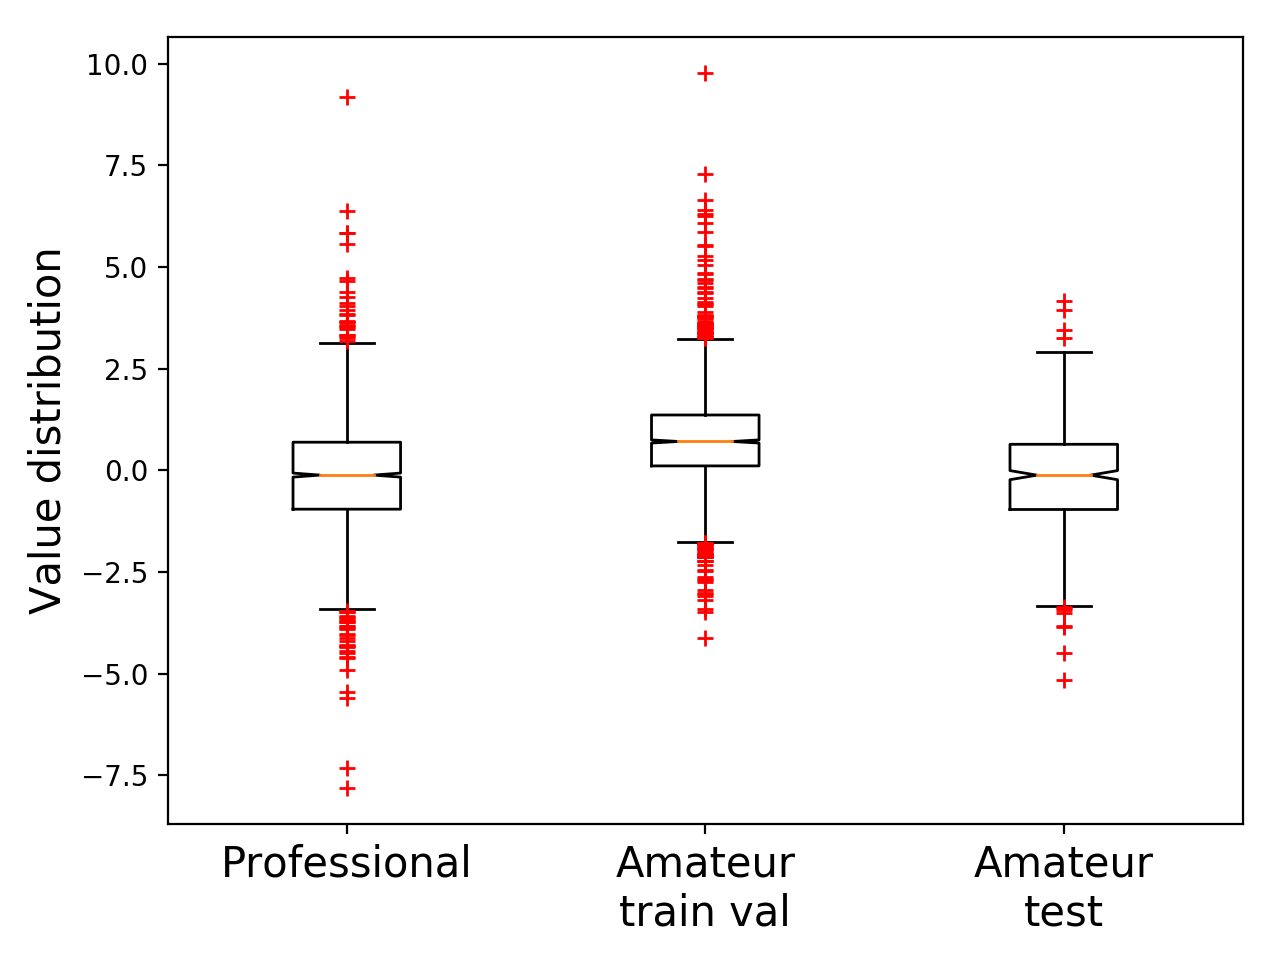
\includegraphics[width=0.475\textwidth]{figs/ch7/nvc_5_lowlevel_erbbands_skewness_mean.png}}
    \hfill

    \subfloat[Bark bands skewness mean]{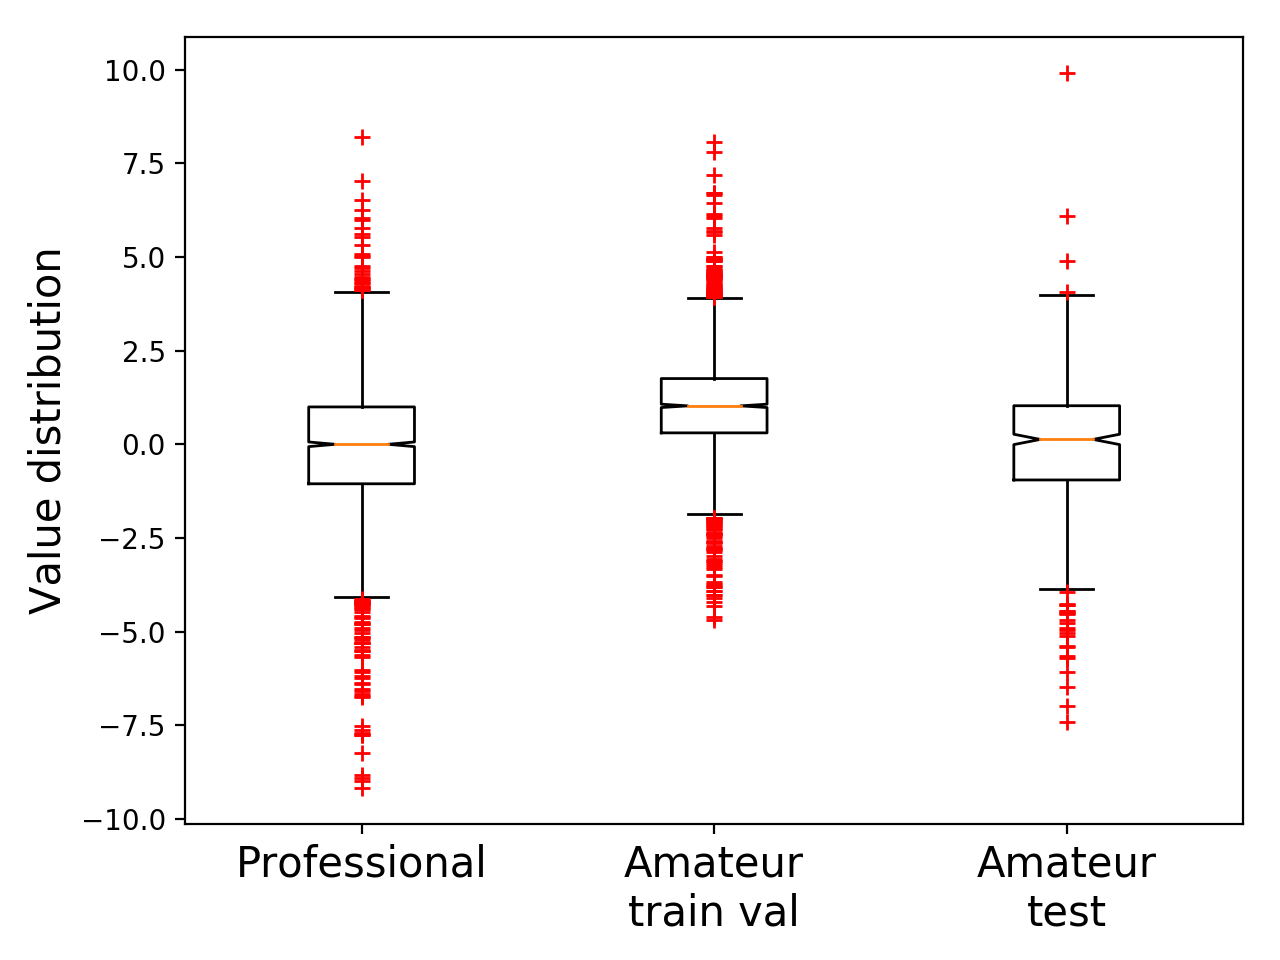
\includegraphics[width=0.475\textwidth]{figs/ch7/nvc_6_lowlevel_barkbands_skewness_mean.png}}
    \subfloat[Spectral complexity std]{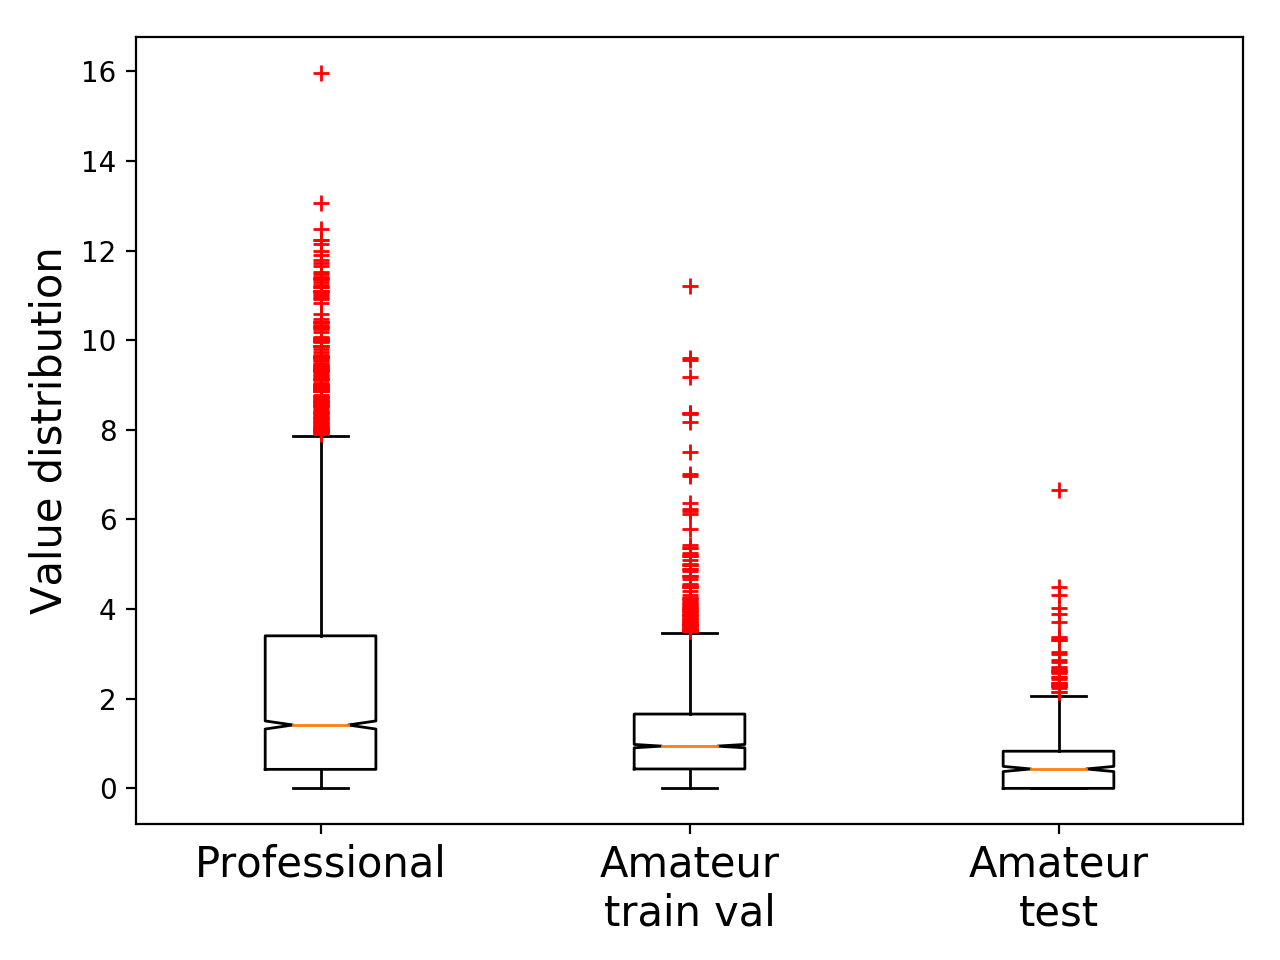
\includegraphics[width=0.475\textwidth]{figs/ch7/nvc_7_lowlevel_spectral_complexity_stdev.png}}

    \caption[Value distributions of the most discriminative features for non-voiced consonant phoneme segments. For the definition of each feature, please consult online.]{Value distributions of the most discriminative features for non-voiced consonant phoneme segments. For the definition of each feature, please consult online\footref{foot:freesound}.}
    \label{fig:ch7:feature_nvc}
\end{figure}
    
\begin{figure}
    \centering
    \subfloat[Phoneme duration]{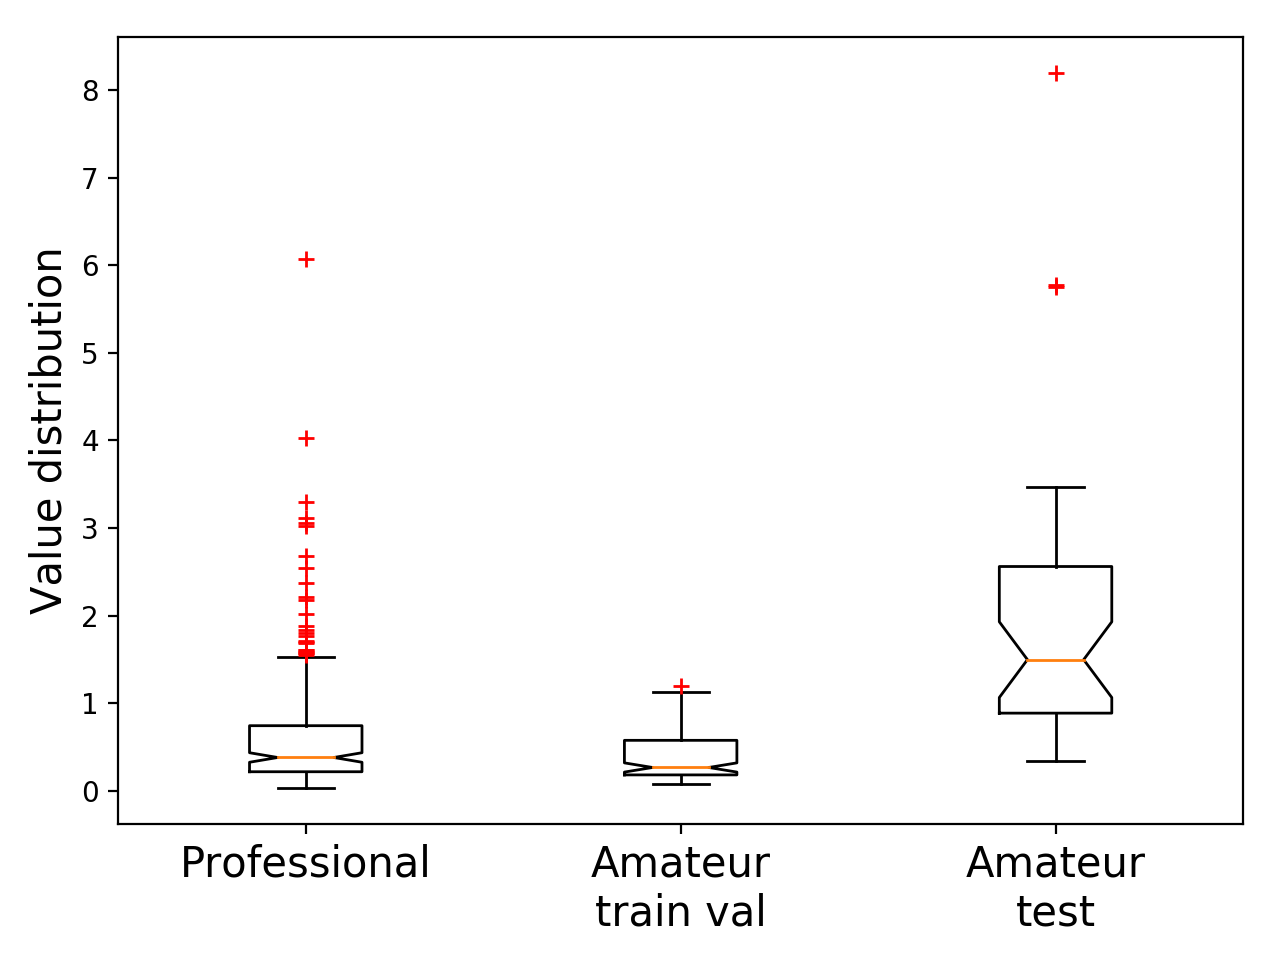
\includegraphics[width=0.475\textwidth]{figs/ch7/O_2_sfx_duration.png}}
    \subfloat[Spectral RMS mean]{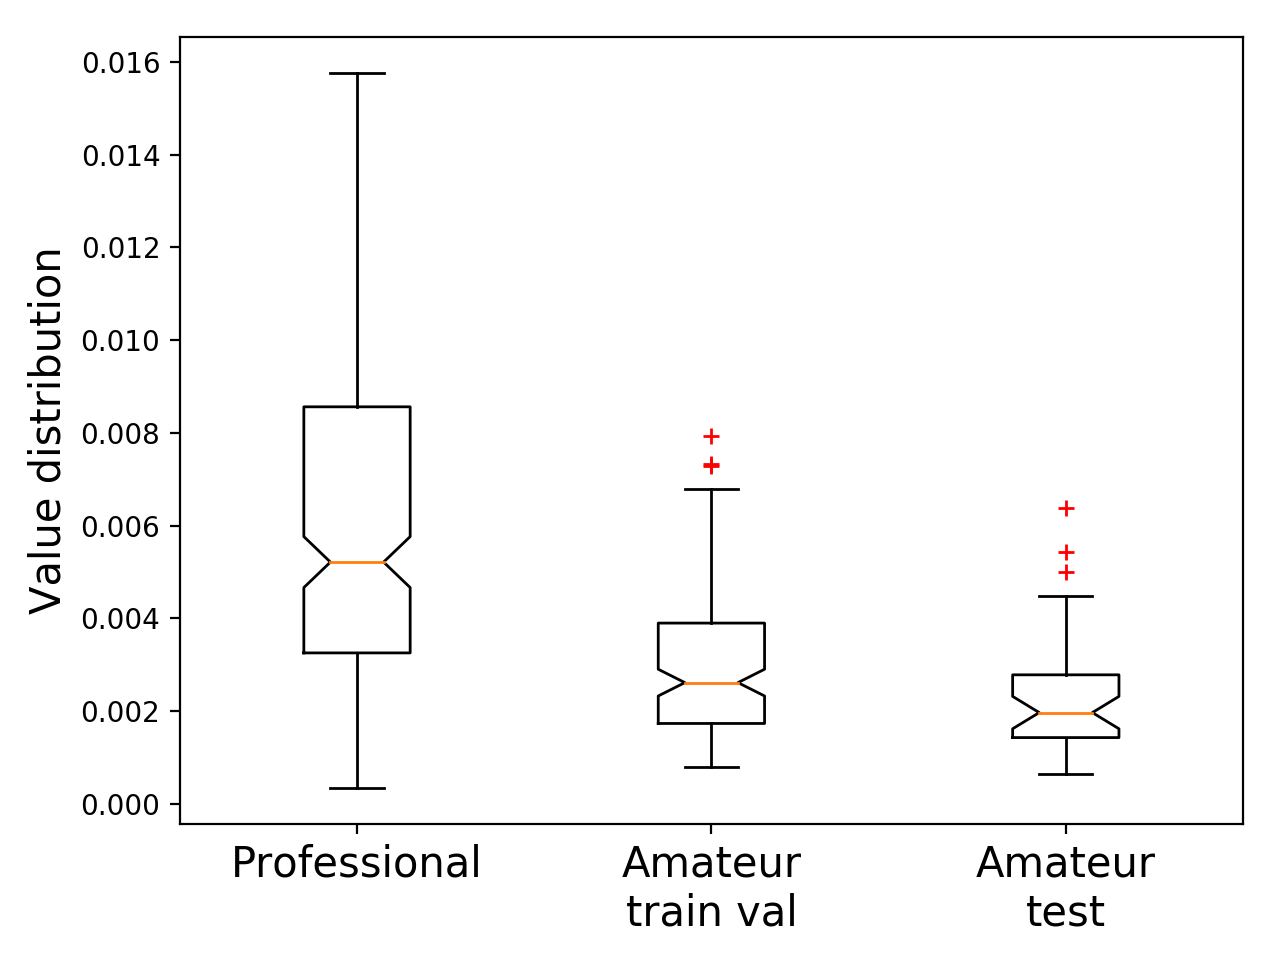
\includegraphics[width=0.475\textwidth]{figs/ch7/O_5_lowlevel_spectral_rms_mean.png}}
    \hfill
    
    \subfloat[Strong decay]{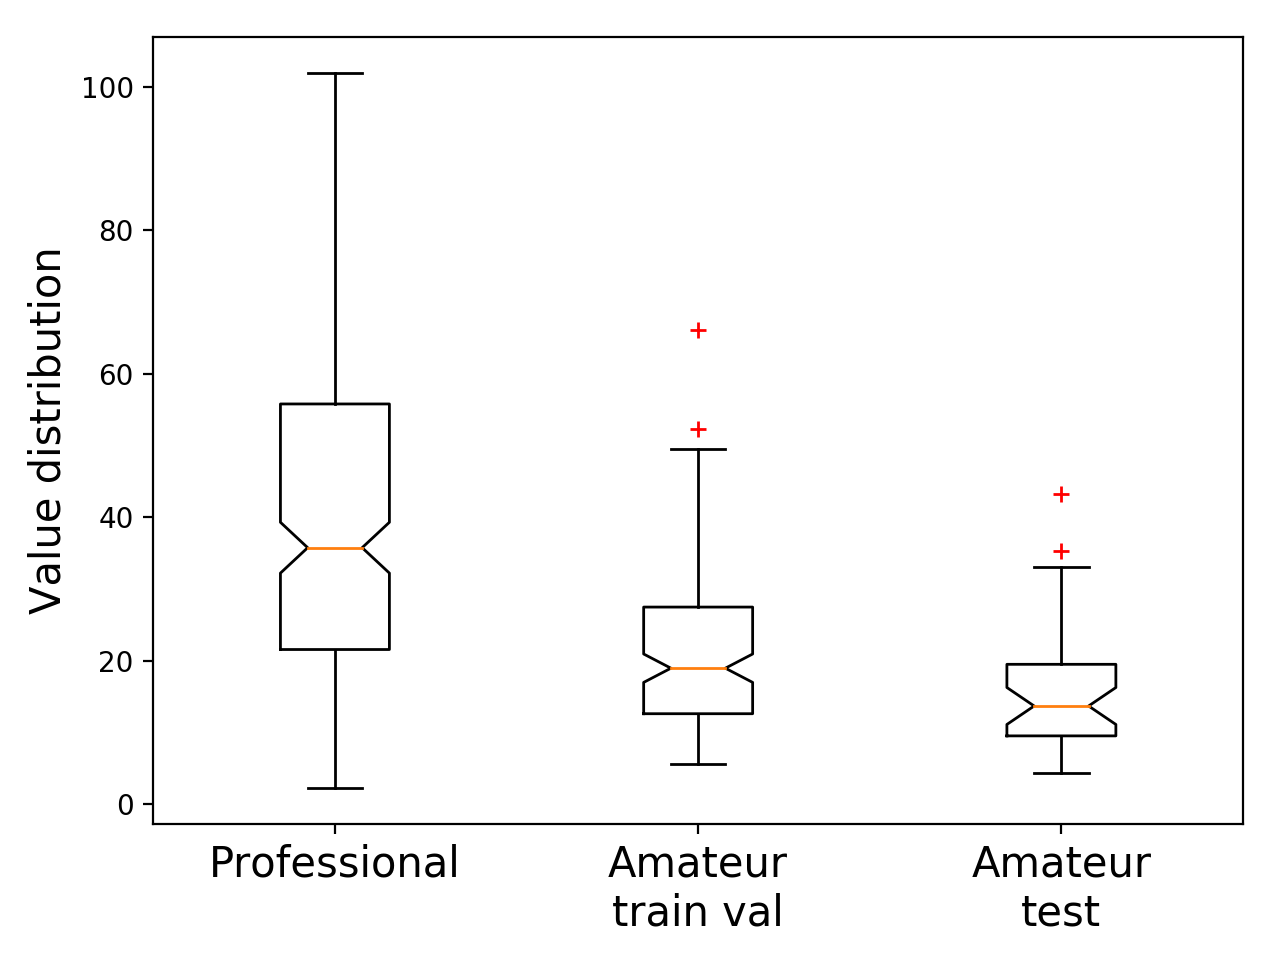
\includegraphics[width=0.475\textwidth]{figs/ch7/O_6_sfx_strongdecay.png}}
    \subfloat[Spectral flux mean]{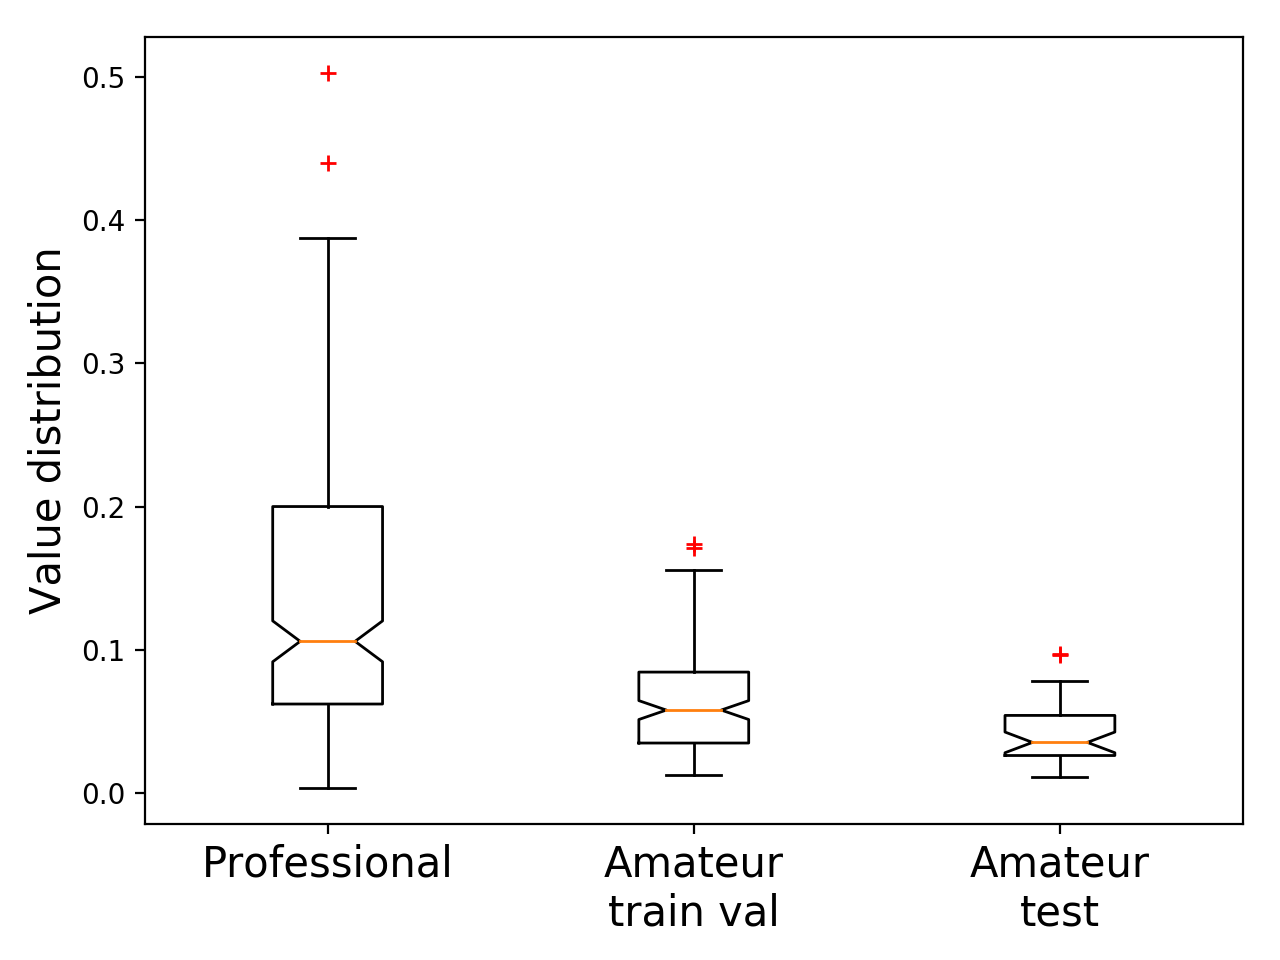
\includegraphics[width=0.475\textwidth]{figs/ch7/O_7_lowlevel_spectral_flux_mean.png}}
    \hfill
    \caption[Value distributions of the most discriminative features for phoneme O segments. For the definition of each feature, please consult online.]{Value distributions of the most discriminative features for ``O" phoneme segments. For the definition of each feature, please consult online\footref{foot:freesound}.}
    \label{fig:ch7:feature_o}
\end{figure}

Figure \ref{fig:ch7:feature_nvc} shows that, for the non-voiced phoneme class, no individual feature can separate the amateur test segments from the professional segments. Figure \ref{fig:ch7:feature_o} indicates that, for the phoneme O class, all these four features can effectively separate the amateur test segments from the professional segments. However, its low test set \gls{AP} (0.667) indicates that the learned phoneme embeddings are far from discriminative. So it is possible that for such phoneme classes, the learned embeddings are overfitted on the train and validation sets, and not discriminative for the test sets. In the next section, we are going to explore four experiments to overcome the overfitting and to improve the phoneme embedding discriminability.

\subsection{Techniques to improve the baseline model}

We explore four experiments to improve the phoneme embedding:

\begin{enumerate}[itemsep=0pt]
\item adding \textbf{attention} mechanism in the network architecture.
\item using \textbf{32 embedding} dimensionality.
\item stacking convolutional layers \textbf{\gls{CNN}} before the \gls{RNN} layers.
\item adding \gls{RNN} input and output \textbf{dropout}.
\end{enumerate}

\textbf{Attention}: The attention mechanism used in this experiment is the same as it has been presented in \secref{sec:ch6:feed_forward_att}.

\textbf{32 embedding}: We consider that the embedding dimension, especially for the overall quality aspect (2-dimensional embedding) is too few to capture sufficient information. To address this problem, we insert an intermediate fully-connected layer with 32 linear activation units between the \gls{RNN} and the output softmax layers. Then we take the 32-dimensional output of this intermediate layer as the embedding.

\textbf{\gls{CNN}}: The architecture of the convolutional layers is similar as it has been presented in \secref{sec:ch6:cnn}. We stack a 6-layers \gls{CNN} between the input and the \gls{RNN} layer. Table \ref{table:ch7:cnn} shows the \gls{CNN} architecture. 

\begin{table}[ht!]
\centering
\caption{6-layers \gls{CNN},  ``8x $1\times3$ \gls{ReLU}" means 8 kernels of which each convolves on 1 frequency bins and 3 temporal frames, using \gls{ReLU} activation function.}
\label{table:ch7:cnn}
\begin{tabular}{c}
\toprule
3 \gls{Conv} 8x $1{\times}3$ \gls{ReLU}\\
Max-pooling $1{\times}3$ \\
3 \gls{Conv} 16x $1{\times}3$ \gls{ReLU}\\
Max-pooling $1{\times}3$ \\
\bottomrule
\end{tabular}
\end{table}

\textbf{Dropout}: To overcome the overfitting, we experiment 0.5 rate dropout for both input and output of the \gls{RNN}.

\subsection{Results and discussion of the improved model}

Figure \ref{fig:ch7:improved_test} shows the results of the four experiments. For the pronunciation aspect, the attention, \gls{CNN} or dropout improves the \gls{AP}. 32 embedding performs worse than the original 29 dimensions, which indicates that increasing the embedding dimensionality cannot always bring the improvement. By combing attention, \gls{CNN} and dropout, we obtain the best \gls{AP} 0.753 on the test set (best combination). For the overall quality aspect, the 32 embedding and \gls{CNN} improves the \gls{AP}. However, combine these two architectures cannot bring improvement than using only 32 embedding. Another observation is that dropout failed in improving the overall quality embedding. Thus it probably doesn't help improve the generalization ability of this embedding.

\begin{figure}[ht!]
    \centering
    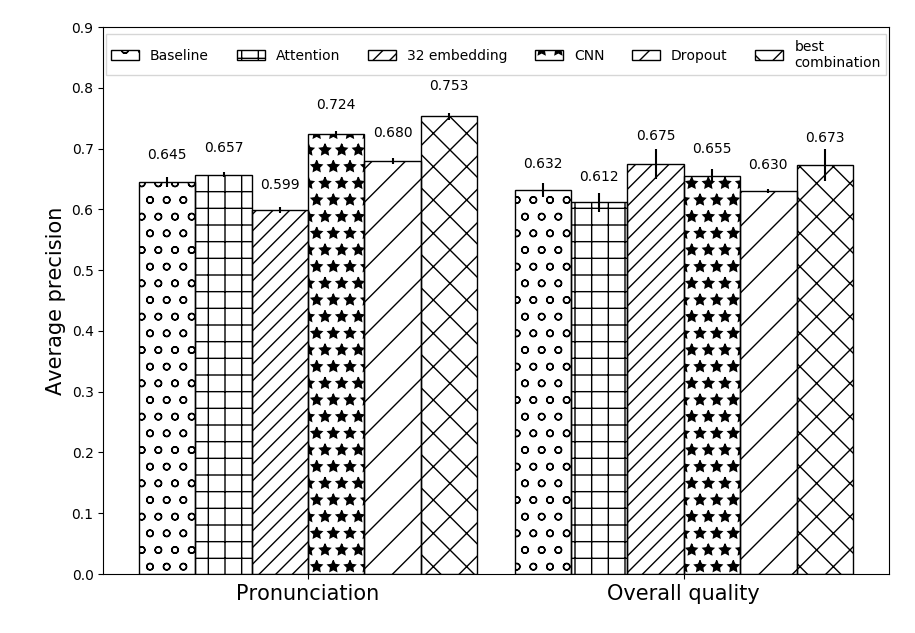
\includegraphics[width=\textwidth]{figs/ch7/improved_test_results_dlfm.png}
    \caption{Average precision on the test set over 5 runs, using optimal classification networks (baseline), and four architectures to improve the baseline. The best combination of pronunciation aspect is to combine attention, CNN and dropout; that of overall quality aspect is to combine 32 embedding and CNN.}
    \label{fig:ch7:improved_test}
\end{figure}

Figure \ref{fig:ch7:tsne_dense} shows the \gls{t-SNE} projection of the 32-dimensional overall quality embeddings. For non-voiced consonant phoneme class, we can observe clearly two separated professional and amateur clusters, and many test set amateur segments are distributed in the train and validation sets amateur cluster. 

\begin{figure}[ht!]
        \centering
        \subfloat[Non-voiced consonant phoneme class]{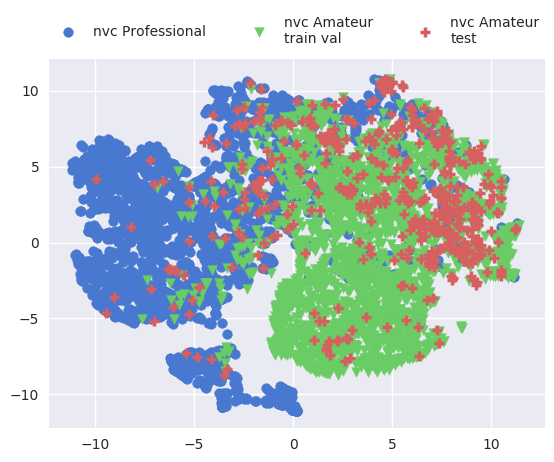
\includegraphics[width=0.475\textwidth]{figs/ch7/nvc_dense.png}\label{fig:tsne_dense_nvc}}
        \subfloat[Phoneme O class]{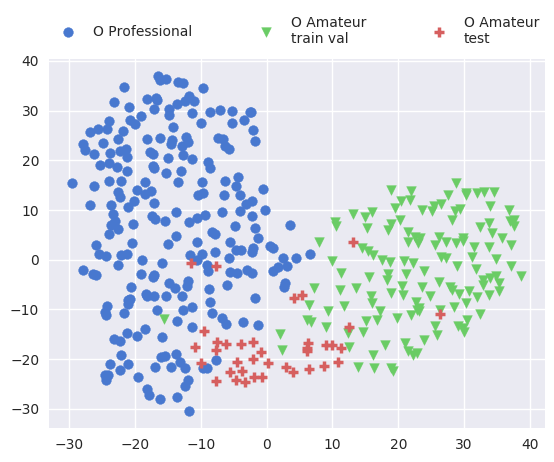
\includegraphics[width=0.475\textwidth]{figs/ch7/O_dense.png}\label{fig:tsne_dense_o}}
            
        \caption[]{t-SNE projection of classification network 32 dimensional phoneme embeddings for overall quality. nvc: non-voiced consonant; Blue dots: phoneme embeddings of the professional singers; Green triangles: training and validation sets phoneme embeddings of the amateur singers; Red plus: test set phoneme embeddings of the amateur singers.}
        \label{fig:ch7:tsne_dense}
    \end{figure}

We can also notice that, for phoneme O class, most of the test set amateur segments are no longer mixed up within the professional cluster, although some segments lie on the border between the professional and the amateur clusters. It worth to notice that the amateur segments in the train and validation sets are entirely composed by the singing samples of the primary school students, while the professional segments are entirely composed by the recordings of the adult singers. The segregation between the amateur test segments and the professional segments means that the model is not overfitted by the age of the singers. Additionally, compared to figure \ref{fig:ch7:tsne_nodense}, 32 dimensional embedding presents a remarkable improvement in separating professional and amateur groups for these two phoneme classes.

\begin{landscape}
\mbox{}\vfill
\begin{figure}[ht!]
    \centering
    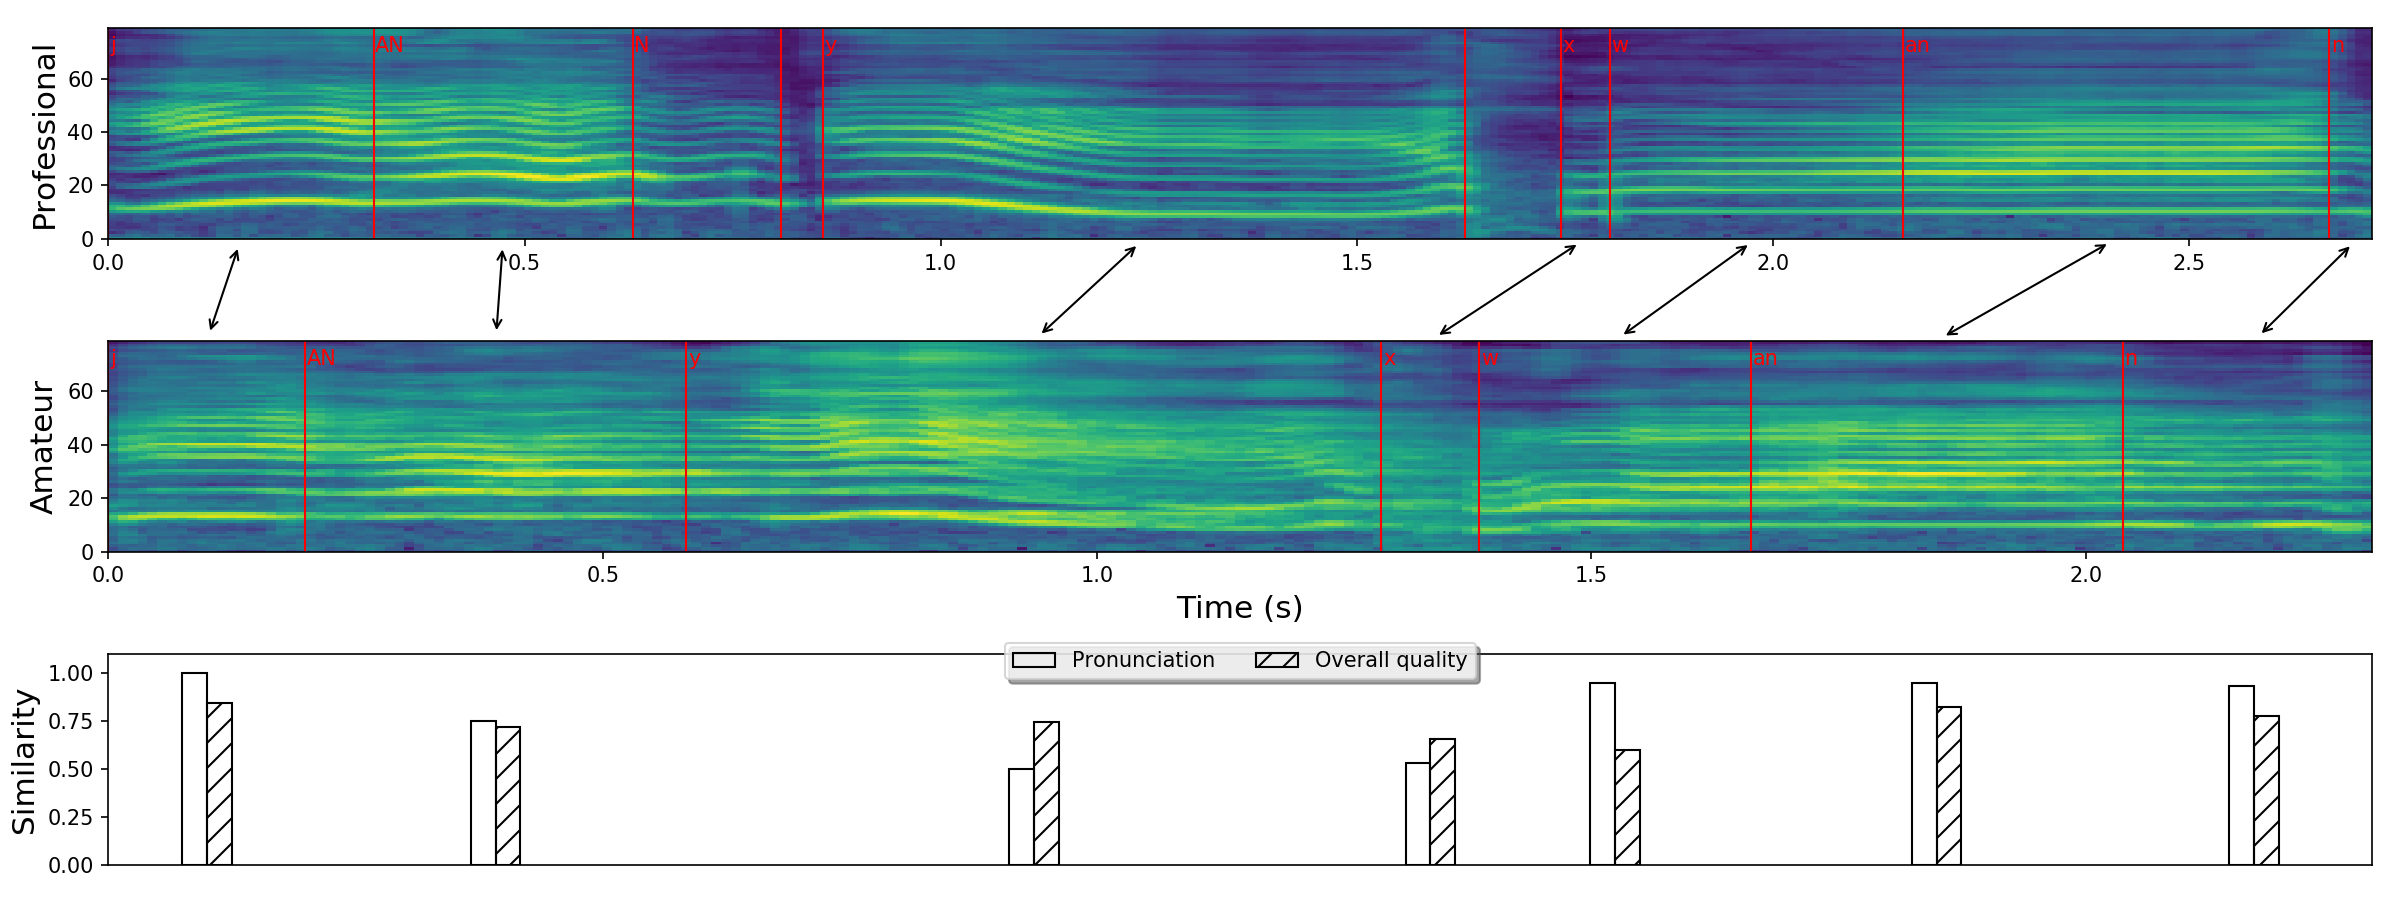
\includegraphics[width=1.5\textwidth]{figs/ch7/yang_yu_huan.png}
    \caption{Illustration of the similarities of embeddings used in grading the singing phonemes on a singing excerpt of three syllables -- yang yu huan. First row: professional singing log-mel spectrogram; Second row: amateur singing log-mel spectrogram; Third row: pronunciation and overall quality similarities by comparing the corresponding professional and amateur phonemes. Vertical red lines: phoneme onsets. Red label following the vertical line is the phoneme name in XSAMPA format.}
    \label{fig:ch7:illustration_embedding}
\end{figure}
\vfill
\end{landscape}

Figure \ref{fig:ch7:illustration_embedding} shows the similarity measurement results by using the phoneme embeddings to grade the amateur singing at phoneme-level. We measure the cosine similarity between the professional and amateur corresponding phoneme embeddings, and ignore the extra or missing phonemes, e.g., the third phoneme ``N" in the professional singing. The pronunciation and overall quality similarity of each phoneme segment are indicated in the third row of the figure. The similarity measures have a potential application for the automatic assessment of jingju singing voice in online education scenario, where the visualization feedback of the pronunciation and overall quality similarities could be an effective guidance for the students to improve their singing.

\section{Siamese phoneme embedding networks}

Siamese network is a network architecture which receives multiple inputs, and shares the same weights. It uses a contrastive loss to learn the similarity between multiple inputs. This network architecture is more complicated than the classification network. However, it outperforms the classification network in learning speech word acoustic embeddings \cite{Settle2016a}. Additionally, the siamese network and the contrastive loss have been initially proposed to learn the similarity between multiple inputs, such as the similarity between images or sounds, which is coherent with the task we are dealing with -- to model the pronunciation and overall quality similarities between phonemes. Thus in this section, we explore the performance of the siamese network on singing voice phoneme embedding. 

\subsection{Semi-supervised Siamese network}

Figure \ref{fig:ch7:siamese_net} illustrates an example of the siamese network experimented in this work for learning the overall quality embedding.

\begin{figure}[ht!]
    \centering
    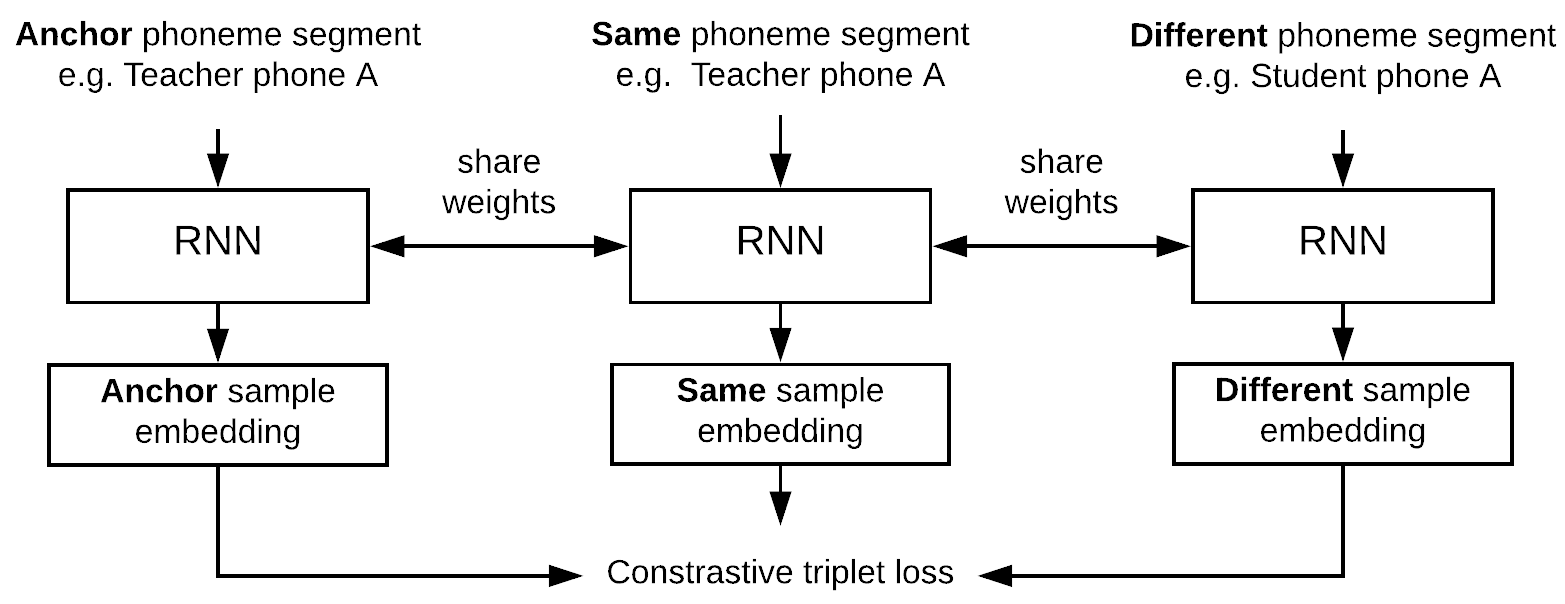
\includegraphics[width=\textwidth]{figs/ch7/siamese_net.png}
    \caption{Semi-supervised siamese phoneme embedding network example for learning overall quality aspect.}
    \label{fig:ch7:siamese_net}
\end{figure}

The network receives three inputs -- \textbf{anchor}, \textbf{same} and \textbf{different}. For instance, we can feed a \textit{teacher phoneme class A} sample into the \textbf{anchor} input, another \textit{teacher phoneme class A} sample into the \textbf{same} input, and a \textit{student phoneme class A} sample into the \textbf{different} input. We disclose the teacher or student labels in this example only for clarifying the network training process. However, in the actual case, we don't need to know the exact labels of these samples, but instead the fact that the \textbf{anchor} and \textbf{same} samples belonging to the same class and the \textbf{anchor} and \textbf{different} samples belonging to different classes, which is also why we name it the semi-supervised network. 

The network outputs are the embeddings for the three input samples -- $x_a$, $x_s$ and $x_d$. Then we use contrastive triplet loss (also known as cos-hinge triplet loss) to minimize the cosine distance between the \textbf{anchor} $x_a$ and \textbf{same} $x_s$ embeddings, and maximize the cosine distance between the \textbf{anchor} $x_a$ and \textbf{different} $x_d$ embeddings. The formula of the contrastive triplet loss is:

\begin{equation}
l = \textrm{max}\{0,m-d_{cos}(x_a, x_s)-d_{cos}(x_a, x_d)\}
\end{equation}

where $d_{cos}(x_1, x_2)$ is the cosine distance between $x_1$ and $x_2$, and $m$ is margin parameter that will be optimized by using the validation set.

To learn the pronunciation embeddings, we only need to feed the network different training samples. For example, a valid training sample combination could be a \textit{phoneme of class A} for the \textbf{anchor} input, another \textit{phoneme of class A} for the \textbf{same} input, and a \textit{phoneme of class B} for the \textbf{different} input.

\subsection{Model training}

We use $N$ \textbf{anchor} samples, where $N$ is the sample number of the training set, then randomly choose another $N$ examples which each match the word of a corresponding \textbf{anchor} sample, then choose another $5N$ random samples for \textbf{different} class to their corresponding \textbf{anchor} samples. This training data sampling strategy leads to $N$ training sample buckets, each includes 5 triplet combinations, where each \textbf{anchor} and \textbf{same} sample pair are repeated 5 times to match with the $5$ \textbf{different} samples. Then we calculate the contrastive triplet loss for each 5 samples combination, and choose the one with the maximum loss to update the network weights. By doing this, we choose the most similar \textbf{different} sample for each \textbf{anchor} sample. This sampling strategy is recommended by S. Settle \cite{Settle2016a} through a personal communication. It has been provided by him that this strategy improved the performance of training speech word acoustic embedding.

\subsection{Experimental setup}

We train two phoneme embedding models respectively for pronunciation and overall quality similarities. The optimal architectures are used directly for the evaluation of the siamese network -- a 2 layers \gls{BiLSTM} architecture for pronunciation similarity and a single layer \gls{BiLSTM} architecture for overall quality similarity. The evaluation procedure and metrics are the same as they have been mentioned in \secref{sec:ch7:experimental_setup_classification}. To find the best-performed margin parameter $m$ for the network, we grid search 5 different values of $m$. Additionally, to test if the network learns useful information, we give the results of the model with randomly initialized weights.

\subsection{Results and discussion}

Table \ref{tab:ch7:margin_search} shows a much inferior performance on the validation set compared with the classification network embeddings (\tabref{tab:ch7:validation_classification}), and the best-performed margin parameter $m=0.15$. 

\begin{table}[ht!]
\centering
\caption{Mean value of average precision on the validation set over 5 runs, using siamese network with the optimal architectures. $m$: margin parameter.}
\label{tab:ch7:margin_search}
\begin{tabular}{lcc}
\toprule
$m$  & Pronunciation AP & Overall quality AP \\
\midrule
0    & 0.275            & 0.507              \\
0.15 & \textbf{0.354}   & \textbf{0.511}     \\
0.3  & 0.332            & 0.508              \\
0.45 & 0.323            & 0.510              \\
0.6  & 0.279            & 0.510             \\
\bottomrule
\end{tabular}
\end{table}

Then we show in the \figref{tab:ch7:validation_classification} the results of the siamese network model on the test dataset, along with the baseline classification model and the siamese network model with random weights. We can observe that (1) the classification embedding outperforms the siamese embedding in a large margin; (2) the siamese network with random weights performs equally than the trained siamese network for the overall quality aspect.

\begin{figure}[ht!]
    \centering
    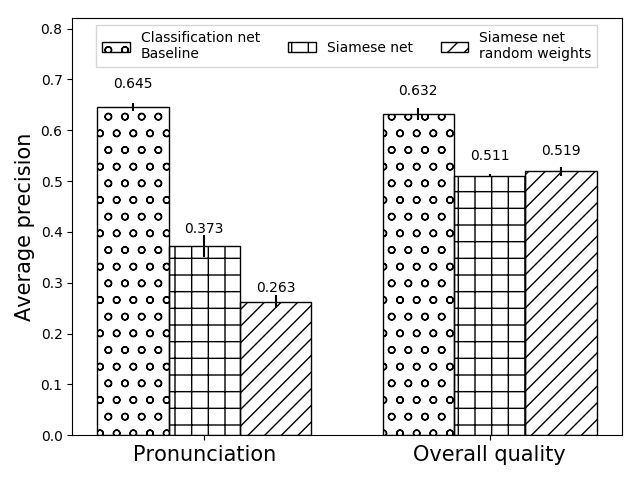
\includegraphics[width=\textwidth]{figs/ch7/baseline_test_results_dlfm.png}
    \caption{Average precision on the test set over 5 runs, using optimal network architectures and margin parameter $m=0.15$.}
    \label{fig:ch7:baseline_test}
\end{figure}

The observation (1) is contradicted by the results in paper \cite{Kampera,Settle2016a}, where they found that siamese network consistently works better than the classification network in learning speech word embedding. A possible reason could be singing voice, especially jingju, is quite different from the speech in terms of the pitch range, spectral variation, syllable or phoneme duration, etc. Another possible reason could be that the training set used for training siamese word embedding (100k word segment pairs) is much larger than our jingju phoneme segment training set (12.5k phoneme segment pairs). We have tried to increase the training set by creating more phoneme segment pairs, however, this makes the training too long to iterate one train-validation loop, which also indicated that siamese network is much hard to train to obtain the equal performance than the classification network. The observation (2) shows that the trained siamese network doesn't learn any useful information for overall embedding. This is contra-intuitive such that we thought that there should have mistakes in the network training, e.g., mistakenly selected \textbf{same} or \textbf{different} samples. However, for the pronunciation aspect, the trained siamese embedding works better than the random weights one, and they use the same experiment pipeline except for the training data preparation step. We examined the data preparation step, and confirmed that in both pronunciation and overall quality aspects, we fed to the network the correct samples and ground truth labels. Thus, the application of learning a siamese network-based phoneme embedding model needs further study.

\section{Conclusions}

This chapter presented a detailed formulation of the task of pronunciation and overall quality similarities measure in jingju singing voice. The approaches utilized the deep learning-based classification and siamese network models to generate phoneme embeddings, and then calculated the similarity measure for jingju singing phonemes. The evaluation of the specific testing dataset showed the possibility of this approach and its limitations. The work presented in this chapter is evaluated on the manually pre-segmented phoneme segments. Thus a future study needs to be carried out for the joint phoneme segmentation and similarity measure.

We mainly addressed the problem of similarity measurement by using fixed-length phoneme embeddings. The presented method firstly used a recurrent neural network with the classification objectives to obtain the phoneme embeddings, then calculated the cosine distance between two embeddings as the similarity measure. Additionally, we experimented with several deep learning techniques aiming to improve the model generalization. As the results, the combination of all the techniques was effective in improving the model performance regarding the pronunciation aspect. While expanding the embedding dimension improved the model performance regarding the overall quality aspect prominently. As an exploration, we also tested the siamese phoneme embedding network since it has been designed for the similarity measurement of multiple inputs. However, the performance was much inferior to the classification model, which requires further study.

For future work, to have an overall assessment of the system pipeline, we will evaluate the similarity measure performance by jointly performing automatic phoneme segmentation and similarity measurement models. The next steps would be investigating deeply in the training data preparation, training speed optimization aspects for the siamese network. 
